
	\tikzset{
	place/.style={
	circle,
	thick,
	draw=black!100, % draw=blue!75,
    % fill=blue!20,
    minimum size=6mm
  },
  extPlace/.style={
    circle,
    dotted,
    draw=black!100, % draw=blue!75,
    % fill=blue!20,
    minimum size=6mm
  },
  extTransition/.style={
    rectangle,
    dotted,
    fill=white,
    minimum width=8mm,
    inner ysep=0.7pt
  },
  transition/.style={
    rectangle,
    thick,
    fill=black,
    minimum width=8mm,
    inner ysep=0.7pt
  },
  extTimedtransition/.style={
    rectangle,
    dotted,
    fill=white,
    minimum width=8mm,
    inner ysep=2pt
  },
  timedtransition/.style={
    rectangle,
    thick,
    fill=white,
    minimum width=10mm,
    inner ysep=2pt
  },
  inhibitor/.style={-o},
  text/.style={}
}
\chapter{Tools}
\label{cha:Tools}
 The development of
these tools used in this work was made using Ubuntu 18.04, wrapping some Linux and Unix
programs/utilities, 100\% compatibility with other operating systems/platforms
was not the primary objective of this part of the work, but can be performed in
some future work. 
The tools developed for this work are available at
\url{https://github.com/Accacio/docsTCC/tree/master/tools}, and the most used
ones will be presented in the following sections.
\section{daoct}
\label{sec:daoct}
To implement the \Autoref{alg:identification}, presented in
\cite{moreira2018enhanced}, a script was created by Ryan Pitanga as part of his
undergraduate project, \cite{pitanga2019modelo}. His code was partially
reimplemented, so it could be used as a command line tool based in common Unix
tools (that uses stdin and
stdout\footnote{\url{http://man7.org/linux/man-pages/man3/stdin.3.html}} to pipe\footnote{\url{http://man7.org/linux/man-pages/man2/pipe.2.html}}
processes).
% Another modification, was to change the \verb|.csv| input file format,
% figure \ref{fig:daoctInput}. The so the
% program could be generic, the names of the variables (inputs and outputs) are in
% the header, making the program more generic.
Some extra features were added, in order to represent the identified model in two
forms: as a graph or as a list.
The graph is represented using the
dot language\footnote{language used by the program graphviz (\url{https://graphviz.org/})
  to draw graphs} and the list represents the \ffunction{} function of the identified automaton. The output in
\verb|.dot| file format can be
input in
another script to draw the state transition diagram of the identified models.
% The \ffunction, as seen in \ref{fig:daoctOutputFfunction}
% An example of the output of the help option can be seen in \Autoref{fig:daoctHelp}

\Autoref{fig:daoctHelp} depicts the help menu of the daoct program. An example of the most common usage of the daoct program can be
presented. Considering the \verb|.csv| file presented in
\Autoref{fig:daoctInput}, it can be input to the daoct program in order to
obtain the paths from the file and identify the \DAOCT{} model. The two outputs
can be obtained by using the following commands: \verb|daoct -i filename.csv -g| and
\verb|daoct -i filename.csv -f|. The first one generates the graph using dot language (shown in
\Autoref{fig:daoctOutput}) and the second one results in the \ffunction{} (shown
in \Autoref{fig:daoctOutputFfunction}). 

% \lstinputlisting[caption=Daoct help
% dialog.,numbers=none,basicstyle=\tiny]{../../figures/tools/daoct/daoctHelp}
% \label{lst:daoctHelp}

\begin{figure}[H]
  \centering 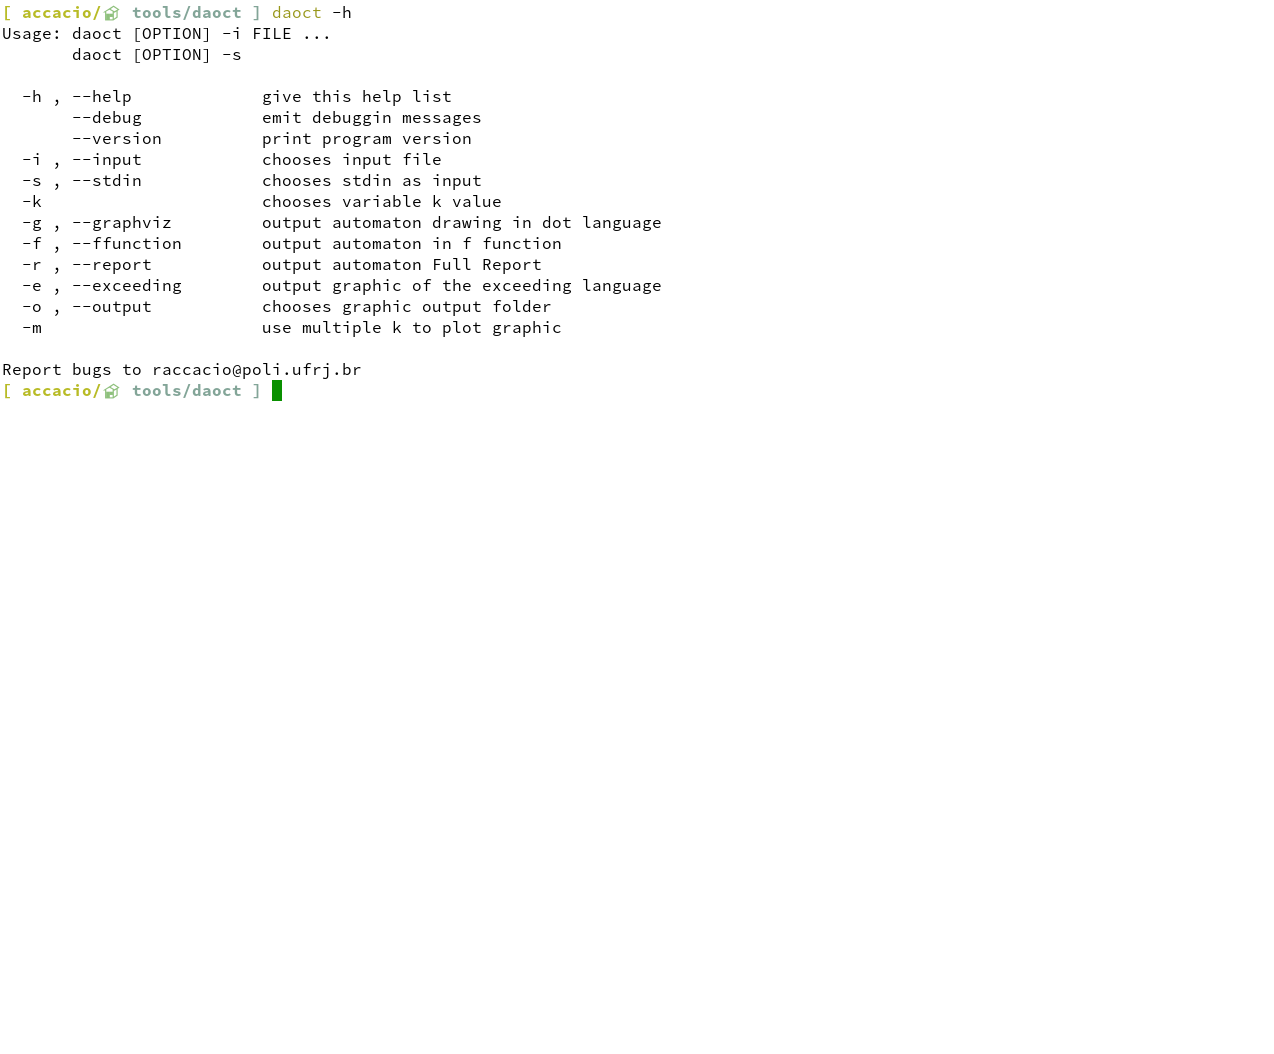
\includegraphics[trim={0 23cm 10cm
    0},clip,width=\textwidth]{tools/daoct/daoctHelp1.png}
  \caption{daoct help dialog.}
  \label{fig:daoctHelp}
\end{figure}
\
% An example of a csv input and the script's different outputs can
% be seen in the following figures:
\vspace{-1cm}
\begin{figure}[H]
\begin{minipage}[H]{0.5\textwidth}
  \centering 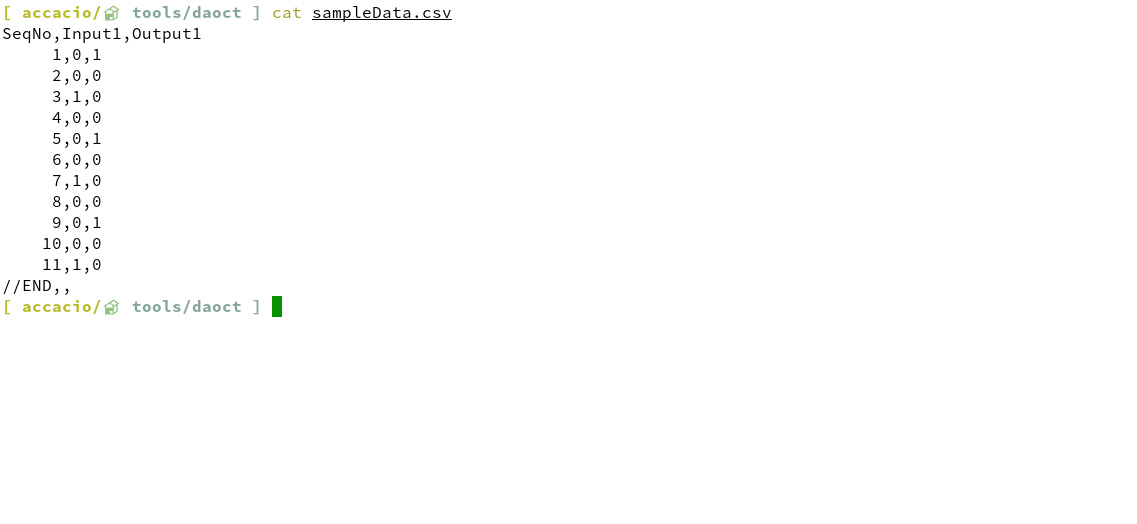
\includegraphics[trim={0 21cm 26cm
    0},clip,width=1.1\textwidth]{tools/daoct/daoctInput.png}
  \caption{daoct csv input file.}
  \label{fig:daoctInput}
\end{minipage}
\begin{minipage}[H]{0.5\textwidth}
  \centering 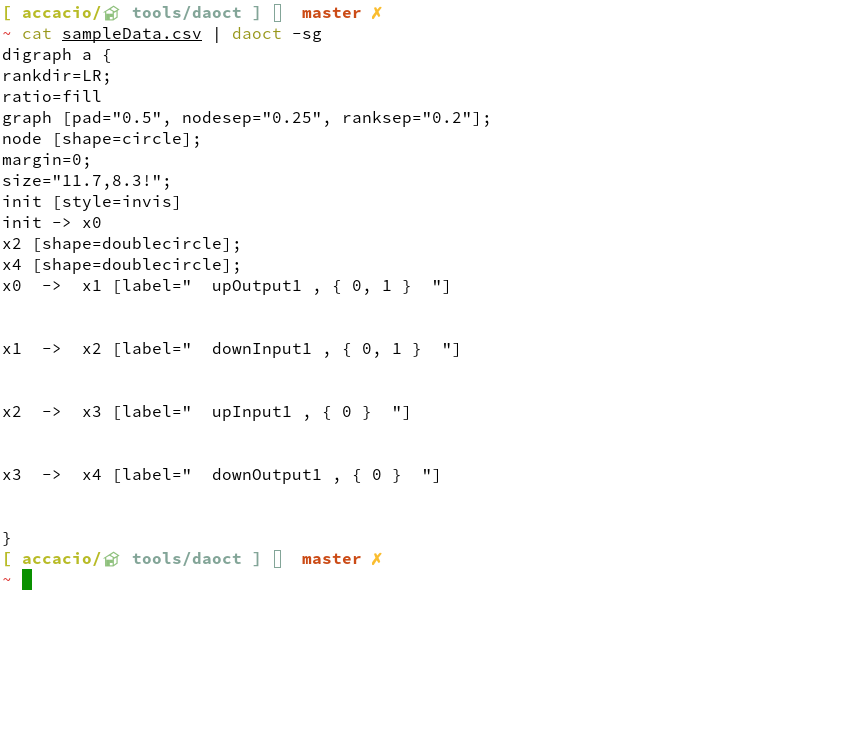
\includegraphics[trim={0 21cm 26cm
    0},clip,width=1.1\textwidth]{tools/daoct/daoctOutput.png}
  \caption{daoct graphviz output.}
  \label{fig:daoctOutput}
\end{minipage}
\end{figure}  

\begin{figure}[H]
  \centering
  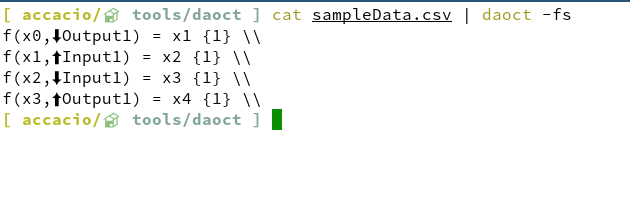
\includegraphics[trim={0 32cm 26cm
    0cm},clip,width=0.5\textwidth]{tools/daoct/daoctOutputFfunction.png}
  \caption{daoct \ffunction{} function output.}
  \label{fig:daoctOutputFfunction}
\end{figure}

% \lstinputlisting[caption=daoct
% main,language=Python]{../../tools/python/DAOCT/daoct}

% \definecolor{keywordstyle}{rgb}{0,1,0.82} \lstinputlisting[caption=daoct
% ,language=Python]{../../tools/python/DAOCT/daoct.py}

% \lstinputlisting[caption=Utils
% ,language=Python]{../../tools/python/DAOCT/utils.py}

% \lstinputlisting[caption=Automaton
% ,language=Python]{../../tools/python/DAOCT/automaton.py}

\section{dot2automata}
\label{sec:dot2automata}

In order to visualize the output of the daoct program, the script \verb|dot2automata| was
created. This program is basically a wrapper of the \verb|dot2tex| program, that is capable of
transforming a \verb|.dot| file into a \verb|.tex| file using tikz syntax. The
program \verb|dot2automata|
pre-process the \verb|.dot| file so the tikz output can be drawn using an automaton style
with states, marked states and labelled arcs, similar to the style presented in \cite{moreira2018enhanced}.
\autoref{fig:dot2automataHelp} shows the help menu of the \verb|dot2automata|
program, describing how to operate it. 
\tikzset{every node/.style={align=center}}

\begin{figure}[H]
  \centering
  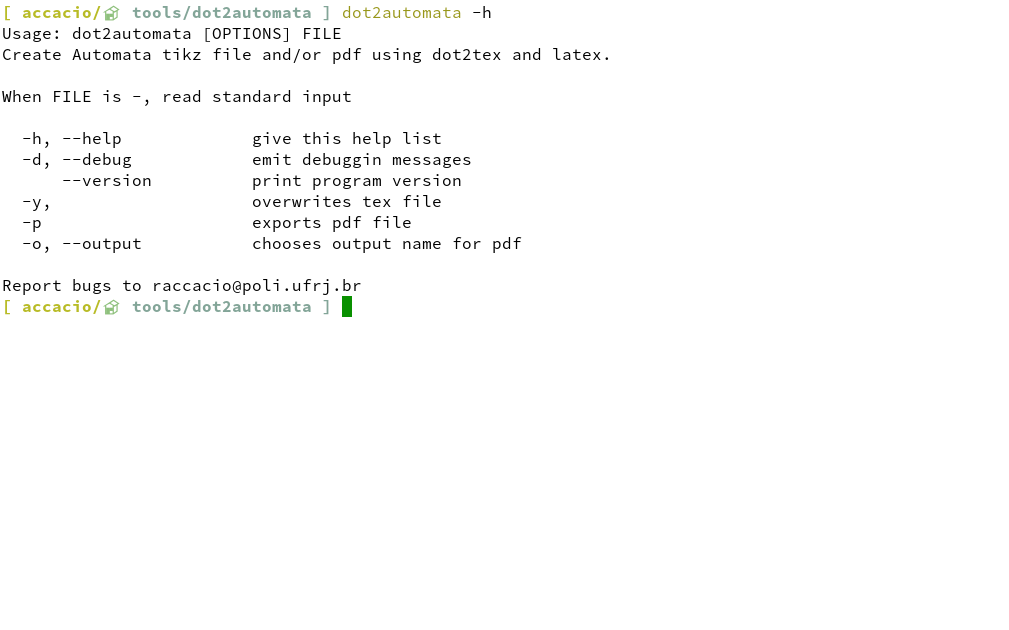
\includegraphics[trim={0 10cm 5cm
    0},clip,width=\textwidth]{tools/dot2automata/dot2automataHelp.png}
  \caption{dot2automata Help.}
  \label{fig:dot2automataHelp}
\end{figure}

The output of the program \verb|daoct| can be piped to the \verb|dot2automata|
program in the following manner: \verb]daoct -i filename.csv -g | dot2automata - -o outputFilename]

This program outputs a \verb|.tikz| file, but it can also output a \verb|.pdf| file. The
\verb|.pdf| file is used as a preview
of the image that is generated by the tikz figure. The tikz figure can be
included in a \LaTeX{} document and resized using the
tikzscale package. So, including a \verb|.tikz| file in a \LaTeX{} document, as
in \autoref{lst:Includetikz}, it can
result in the diagram depicted in \autoref{fig:Dot2automataSampleOutput}.

\lstset{%
  % basicstyle=\small\ttfamily,
  language=[LaTeX]{TeX}
}
\begin{lstlisting}[caption=Include tikz file.,label={lst:Includetikz},numbers=none]
\begin{figure}[H]
  \centering
  \includegraphics[width=\textwidth]{tools/dot2automata/sampleData.tikz}
  \caption{dot2automata output.}
\end{figure}
\end{lstlisting}
\begin{figure}[H]
  \centering
  \includegraphics[width=\textwidth]{tools/dot2automata/sampleData.tikz}
  \caption{dot2automata output.}
  \label{fig:Dot2automataSampleOutput}
\end{figure}


% \lstinputlisting[caption=configPetriNet,language=bash]{../../tools/bash/configPetriNet}

% \lstinputlisting[caption=dot2automata,language=bash]{../../tools/bash/dot2automata}

% \lstinputlisting[caption=dot2petri,language=bash]{../../tools/bash/dot2petri}

% \lstinputlisting[caption=linkPetriNets,language=bash]{../../tools/bash/linkPetriNets}

% \lstinputlisting[caption=linkTables,language=bash]{../../tools/bash/linkTables}

% \lstinputlisting[caption=petriml2dot,language=bash]{../../tools/bash/petriml2dot}

% \lstinputlisting[caption=removeVarsFromData,language=bash]{../../tools/bash/removeVarsFromData}

% \lstinputlisting[caption=treatCSV,language=bash]{../../tools/bash/treatCSV}

\section{dot2petri}
\label{sec:dot2petri}

The \verb|dot2petri| program is a similar to \verb|dot2automata|.The 
working principle is the same but the objective is different. For \verb|dot2petri| program, the objective is to
visualize Petri Nets. Its help dialogue is presented in \Autoref{fig:dot2petriHelp}:
\begin{figure}[H]
  \centering
  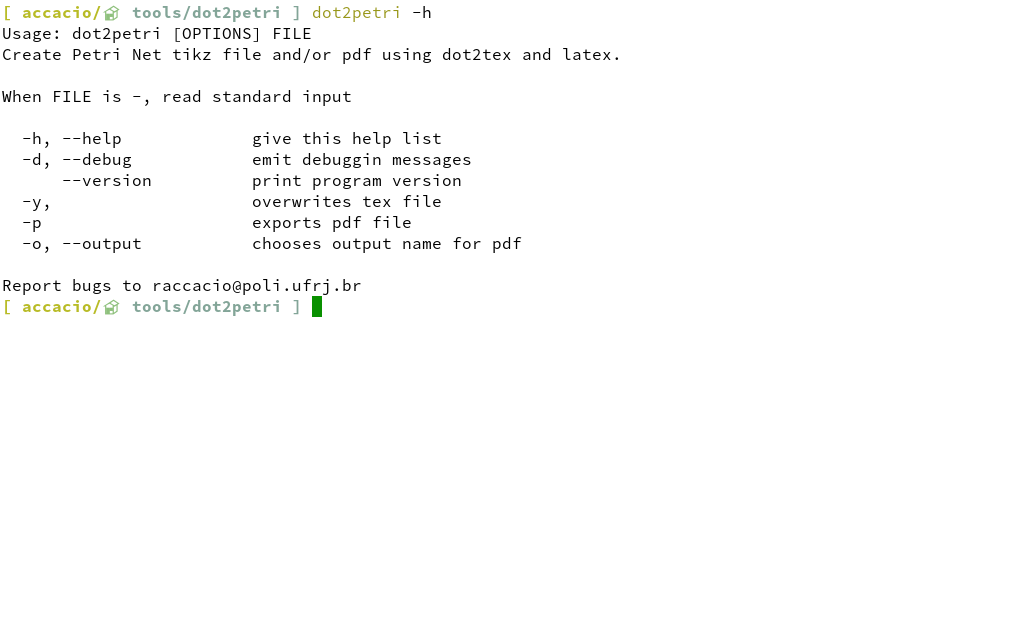
\includegraphics[trim={0 11cm 5cm
    0},clip,width=\textwidth]{tools/dot2petri/dot2petriHelp.png}
  \caption{dot2petri Help.}
  \label{fig:dot2petriHelp}
\end{figure}

The input \verb|.dot| file has a syntax slightly different from \emph{plain vanilla} dot
language, as we can see in the following listing:

\lstinputlisting[caption={dot2petri input dot
  file.},label={lst:dot2petriSampleData},numbers=none,basicstyle=\scriptsize]{../../figures/tools/dot2petri/sampleData.dot}

Using this modified syntax it is easy to define places, marked places,
transitions, timed transitions, and different kinds of arcs. Places are defined
using `p' followed by an identification number. Marked places are similar to
places but have the letter `m' and a number appended, this number represents how
many tokens are in this place. Transitions are defined with a simple `t'
followed by its identification number and timed transitions are created using `tt' and the
id. The arcs can be defined using `->' between two tags (between places and
transitions and vice-versa). An inhibitor arc can be created changing the style
of the arc. A label can be used to represent the $Pre$ and $Post$ functions of the
Petri Net. A tikz style for
external places
and transitions is created in order to be represented by dotted lines. External
places and transitions use the same tags of normal places and transitions, but
with a letter `e' prepended.
% so we can see where different parts interconnect themselves.

Such dot files can be created in two ways: manually writing them or using
another program called \verb|petriml2dot| present in the same repository. The
\verb|petriml2dot| program converts a file in \emph{petriml} format, created using the Platform Independent Petri
net Editor 2 (PIPE2)\footnote{\url{http://pipe2.sourceforge.net/}} into the dot
format.
PIPE2 is a very powerful tool to design Petri Nets, since it is possible to simulate the
net and it can generate reachability graphs, but in its current version, it
lacks a tool to export the graph as a \verb|.tikz| file. So,
\verb|petriml2dot| and \verb|dot2petri| are used to fill the gap.

The code shown in \Autoref{lst:dot2petriSampleData} used as input for the
\verb|dot2petri| script outputs a \verb|.tikz| file. Including the \verb|.tikz| in a similar fashion
to the one shown in \Autoref{lst:Includetikz}, can result in the following figure:
\begin{figure}[H]
  \centering
  \includegraphics[width=0.9\textwidth]{tools/dot2petri/sampleData.tikz}
  \caption{dot2petri output.}
  \label{fig:Dot2automataSampleOutput}
\end{figure}

% \section{Other Scripts}
% \label{sec:otherScripts}
% A couple of other scripts were created to ease the building process. The 
% \verb|linkPetriNets| and \verb|linkTables|, for instance, that together can link tex tables to
% tikz petri net figures, so they can hyperlinked in digital format, as seen in
% \Autoref{fig:petriInitialization}. And other scripts that can pre-process the csv
% tables before sending to \verb|daoct|, as in \verb|treatCSV| and \verb|removeVarsFromData|.


%%% Local Variables:
%%% mode: latex
%%% TeX-master: "../monografia"
%%% End:
